\section{Predicting Employee Behaviour}
\label{sec:predicting}

Predicting employees behaviour is a useful form of analyse for the supplied data.  

\subsection{Simple Model}
\label{sec:simplemodel}
\subsubsection{Defining Locations}
The first step in creating a probabilistic model is to choose the locations that will be used to calculate the probabilities from. \\
\begin{figure}[H]
\centering
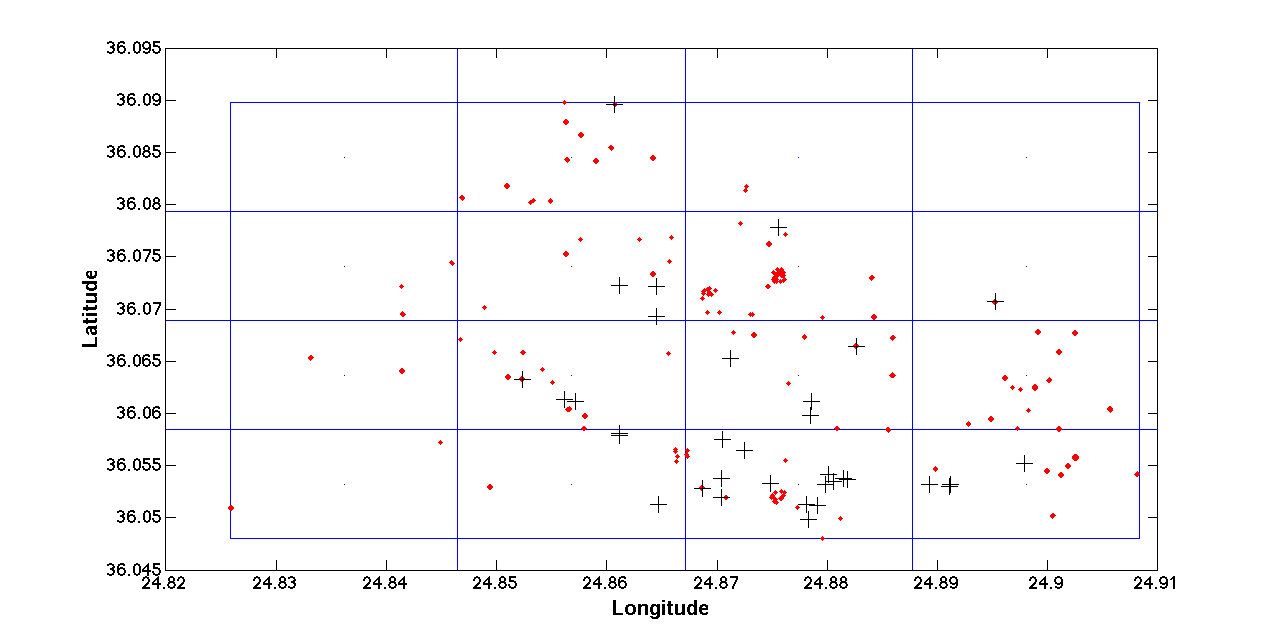
\includegraphics[width=1\textwidth]{locationbound.png}
\caption{\label{fig:locationbound}A graph showing the boundaries created for 16 areas, and the start and end points of all journeys. }

\end{figure}
\noindent This method involves splitting Abila up in to sectors, which is done using the minimum and maximum points from the data, and using these as the boundaries. A set of equidistant points are then selected along the x and y axis, which are used as the corners of the boundaries. From this rectanglar boundaries are created to distinguish between the different regions, as shown in Figure \ref{fig:locationbound}. Each region is labelled and all points that fall within this region are assigned this class. The regions are labelled from 1 to 16 with the lower left corner labelled as 1 and the upper right corner labelled as 16. 

\noindent An important factor with this type of model is to consider how many clusters to use. For the simple model, using 16 clusters in a 4x4 grid is chosen, as there are 34 known locations in the GPS data (see Section \ref{sec:completeloc} ), and if each known location shares a cluster with one other known location, that leaves 17 clusters, to which 16 is the nearest square number.
%Finish this section - I picked 16. Why? What made me do that?

\subsubsection{Calculating Probabilities}

When creating an ideal probabilistic model, the probability of travelling to another location will be dependent on various factors, such as the time of day. A simplified model is assumed, where the probability of an employee travelling to another region is dependent on regions the employee has been before. This is shown in Equation \ref{eq:probtot} :
\begin{equation}\label{eq:probtot}P(l_n | l_{n-1}, l_{n-2}, l_{n-3}, ...),\end{equation}
where $l_n$ is the region of the employee at time $n$. In this model the previous locations of the employee until $n=-\infty$ are taken into account for the probability calculation. As this is impossible to create, an assumption must be made, known as the Markov assumption shown in Equation \ref{eq:markovassumpt}\cite{markov}. %http://di.ubi.pt/~jpaulo/competence/tutorials/hmm-tutorial-1.pdf reference this here
\begin{equation}\label{eq:markovassumpt}P(l_n | l_{n-1}, l_{n-2}, ...)\approx P(l_n | l_{n-1})\end{equation}

\noindent This assumption is a First Order Markov Assumption, which means that only the previous location is considered when calculating the probability.\\
\noindent Using this assumption, the probabilities are calculated by summing the number of journeys from the start region to another end region. This is then divided by the number of journeys from the start point to any point  \cite{gpspredict}.\\ 
%reference gps report here
 

\subsection{Simple Model Analysis}
\label{sec:simpleanalysis}
%You need to do this section, you can't keep putting it off
%Talk about predicting
Predictions using this model can be calculated very simply, as each journey between two points is set a probability. Therefore, if there are four locations; A, B, C and D, the probability of someone travelling from A to B and then from B to C would just be the product of the two probabilities. \\
%Which journey has the highest probability of happening from each cluster?

\subsubsection{Analysing all GPS Data}
\begin{table}[H]
\begin{center}
\begin{tabular}{|l|l|l|}
\hline
Start Position & Most Likely End Position & Probability \\ \hline \hline
1  &   3   & 0.5000 \\ \hline
2  &   11  & 0.6000 \\ \hline
3  &    8  & 0.2207 \\ \hline
4  &    3  & 0.4892 \\ \hline
5  &    5  & 0.5625 \\ \hline
6  &    3  & 0.6939 \\ \hline
7  &    3  & 0.6128 \\ \hline
8  &    4  & 0.6774 \\ \hline
9  &    6  & 0.4615 \\ \hline
10 &    3  & 0.3595 \\ \hline
11 &   10  & 0.2366 \\ \hline 
12 &    3  & 0.6667 \\ \hline
13 &    1  & 0.0000 \\ \hline
14 &   10  & 0.3180 \\ \hline
15 &   11  & 0.5000 \\ \hline
16 &    1  & 0.0000 \\ \hline

\end{tabular}


\caption{\label{table:simplemodel}Results of probability calculations}
\end{center}
\end{table}

As can be seen from Table \ref{table:simplemodel}, the most probable region that people will travel to is 3. This could be explained as region 3 is the region that Gastech is located in. It also has the highest number of establishments that people used their credit cards in.


\noindent  The probabilities for area 16 is equal to 0 because there are no journeys that occur in either of those areas. This could be explained by region 16 being taken up mostly by  the sea.\\
%From work


\noindent In order to see where people are likely to travel from work, region 3 is used as the start point. The probabilities for a journey to each region are shown in Table \ref{table:fromwork}. This table shows that the four areas with the highest probability of being the target location from 3 are 8, 3, 4 and 6. 4 and 8 are the regions that restaurants are located in, so these being the highest probabilities suggests the employees leave work and go straight to a restaurant, whether at lunch or straight after work.

\noindent As for people from region 3 having a high probability of staying within region 3 when they travel, it is likely down to the fact that region 3 is full of places that people use their credit cards.

\begin{table}[H]
\begin{center}
\begin{tabular}{|l|l|}
\hline
End Location & Probability \\ \hline \hline
	1  &  0.0337 \\ \hline
    2  &  0.0000 \\ \hline
    3  &  0.1463 \\ \hline
    4  &  0.1394 \\ \hline
    5  &  0.0012 \\ \hline
    6  &  0.1394 \\ \hline
    7  &  0.0755 \\ \hline
    8  &  0.2207 \\ \hline
    9  &  0.0070 \\ \hline
   10 &  0.0732 \\ \hline
   11  &  0.0767 \\ \hline
   12 &  0.0105 \\ \hline
   13 &  0.0000 \\ \hline
   14  &  0.0767 \\ \hline
   15 &  0.0000 \\ \hline
   16 &  0.0000\\ \hline

\end{tabular}
\caption{\label{table:fromwork}Results of probability calculations from area 3}
\end{center}
\end{table}
